\documentclass[11pt,a4paper]{article}
\usepackage[utf8]{inputenc}
\usepackage[english]{babel}
\usepackage[margin=2.5cm]{geometry}
\usepackage{graphicx}
\usepackage{float}
\usepackage{hyperref}
\usepackage{xcolor}
\usepackage{fancyhdr}
\usepackage{titlesec}
\usepackage{enumitem}

% Define colors
\definecolor{maincolor}{RGB}{45, 52, 54}
\definecolor{accentcolor}{RGB}{74, 144, 226}

% Configure hyperlinks
\hypersetup{
    colorlinks=true,
    linkcolor=accentcolor,
    urlcolor=accentcolor,
    citecolor=accentcolor
}

% Configure headers and footers
\pagestyle{fancy}
\fancyhf{}
\fancyhead[L]{REALLOCATE GeoJSON Tutorial}
\fancyhead[R]{\thepage}
\renewcommand{\headrulewidth}{0.5pt}
\renewcommand{\footrulewidth}{0pt}

% Configure section titles
\titleformat{\section}{\large\bfseries\color{maincolor}}{\thesection}{1em}{}
\titleformat{\subsection}{\normalsize\bfseries\color{maincolor}}{\thesubsection}{1em}{}

% Configure lists
\setlist[enumerate]{itemsep=0.5em}
\setlist[itemize]{itemsep=0.3em}

\title{
    \vspace{-2cm}
    {\Large\bfseries\color{maincolor} REALLOCATE Project}\\
    \vspace{0.5cm}
    {\Huge\bfseries Pilot Location GeoJSON\\Creation Tutorial}\\
    \vspace{0.3cm}
    {\large Guide for Geographic Data Collection}
}

\author{Tiago Tamagusko}
\date{\today}

\begin{document}

\maketitle
\thispagestyle{empty}

\vspace{1cm}

\section*{Overview}

This tutorial provides instructions for creating standardized GeoJSON files containing the pilot location data and corresponding areas of influence for the REALLOCATE project pilots. The methodology employs the web-based \url{http://geojson.io} platform to ensure consistent geographic data collection and formatting across all pilot sites.

\vspace{0.5cm}

\section{Map Editor Initialization}

Navigate to \url{http://geojson.io}. Navigate and zoom to your pilot's city or region to locate the specific area where your pilot is situated.

\begin{figure}[H]
    \centering
    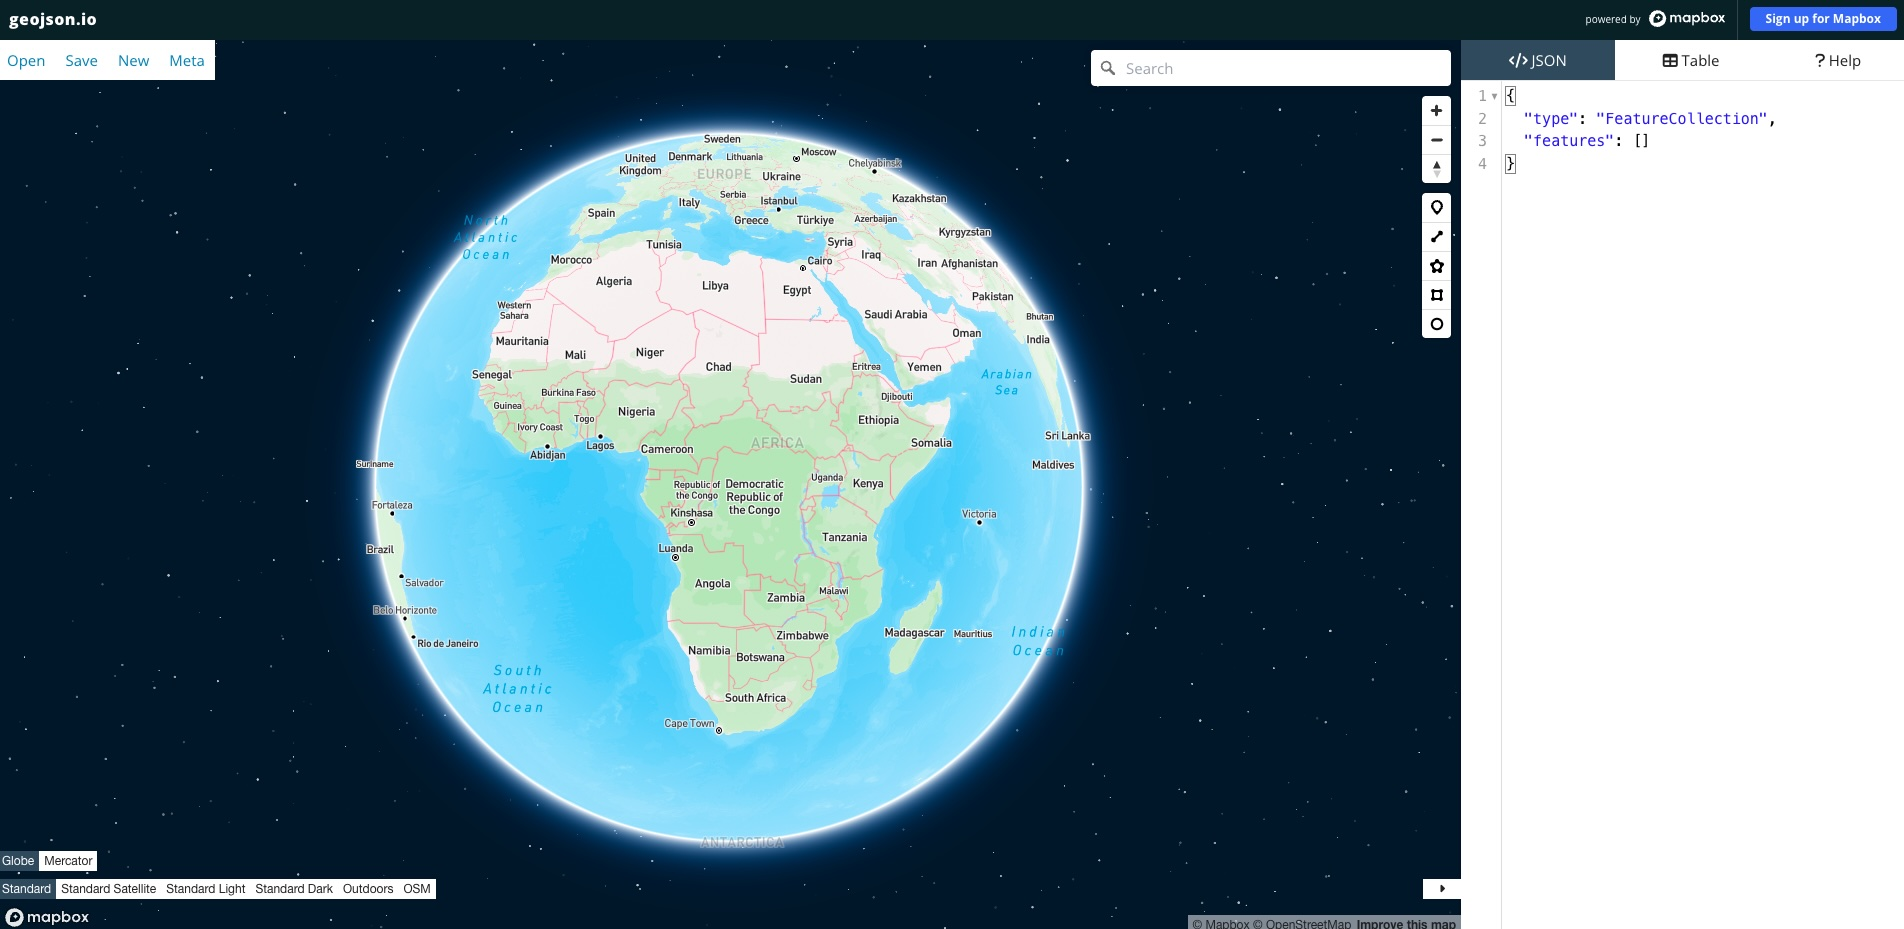
\includegraphics[width=\textwidth]{img/step1.jpg}
    \caption{GeoJSON.io interface showing the global map view with editing tools panel on the right side}
    \label{fig:step1}
\end{figure}

\newpage

\section{Pilot Location Point Creation}

\subsection{Tool Selection}

Access the point creation tool by clicking the \textbf{Draw Point} icon in the right toolbar or use the keyboard shortcut \texttt{m}.

\begin{figure}[H]
    \centering
    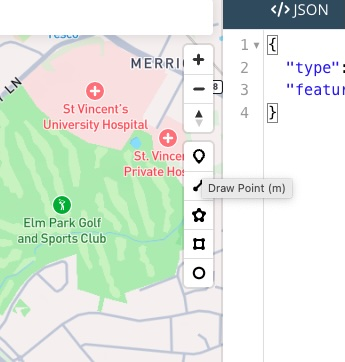
\includegraphics[width=0.6\textwidth]{img/step2_1.jpg}
    \caption{Point drawing tool highlighted in the toolbar interface}
    \label{fig:step2_1}
\end{figure}

\subsection{Geographic Positioning}

Execute a single click on the map at the precise coordinates where your pilot site is located. This action creates a point geometry with geographic coordinates.

\begin{figure}[H]
    \centering
    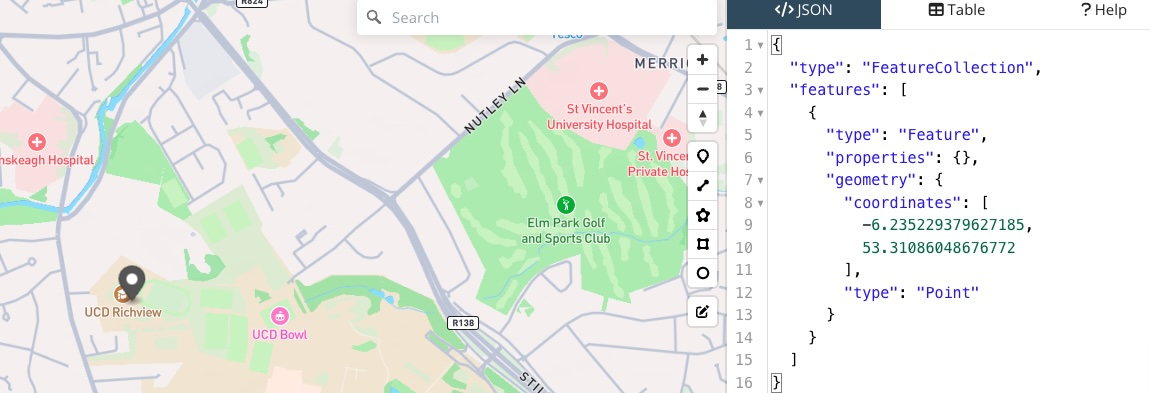
\includegraphics[width=0.95\textwidth]{img/step2_2.jpg}
    \caption{Point marker placed on the map with corresponding GeoJSON coordinates displayed in the code panel}
    \label{fig:step2_2}
\end{figure}

The point coordinates are automatically captured and displayed in the GeoJSON code panel on the right side of the interface.

\section{Area of Influence Polygon Creation}

\subsection{Polygon Tool Activation}

Select the \textbf{Draw Polygon} tool from the right toolbar or utilize the keyboard shortcut \texttt{p}.

\begin{figure}[H]
    \centering
    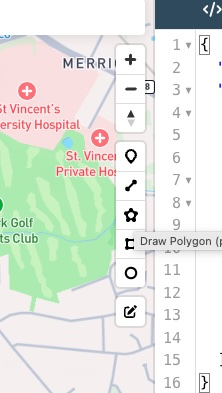
\includegraphics[width=0.4\textwidth]{img/step3_1.jpg}
    \caption{Polygon drawing tool selected in the toolbar}
    \label{fig:step3_1}
\end{figure}

\subsection{Polygon Construction}

Create the area boundary by clicking multiple points around your designated area to form a polygon shape. Complete the polygon by double-clicking on the final point or press enter.

\begin{figure}[H]
    \centering
    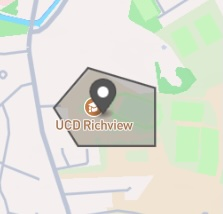
\includegraphics[width=0.5\textwidth]{img/step3_2.jpg}
    \caption{Completed polygon representing the area of influence around the pilot location}
    \label{fig:step3_2}
\end{figure}

The polygon vertices define the precise boundaries of the pilot's area of influence.

\section{Data Export and Validation}

\subsection{File Export Process}

Click the \textbf{Save} button located at the top of the screen and select \textbf{GeoJSON} format from the dropdown menu to download the file.

\begin{figure}[H]
    \centering
    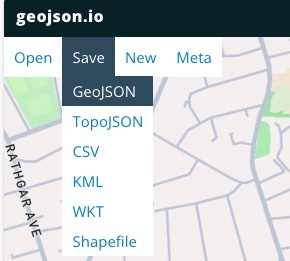
\includegraphics[width=0.6\textwidth]{img/step4.jpg}
    \caption{Save menu displaying GeoJSON format selection option}
    \label{fig:step4}
\end{figure}

\subsection{Data Verification}

Validate the exported file by opening the saved \texttt{.geojson} file in \url{http://geojson.io} using the \textbf{Open} button. Verify that both the pilot point and area of influence polygon are correctly displayed and positioned.

\section{File Submission Protocol}

Compose an email with the following standardized subject format:

\begin{center}
\texttt{REALLOCATE: Pilot Location and Area - [Your City] - [Pilot Name]}
\end{center}

Attach the validated \texttt{.geojson} file and send to:
\begin{itemize}
    \item \texttt{tiago.tamagusko@ucd.ie}
    \item \texttt{ungku.sonet@ucd.ie}
\end{itemize}

\section*{Technical Specifications}

\begin{itemize}
    \item \textbf{Coordinate System:} WGS84 (EPSG:4326)
    \item \textbf{File Format:} GeoJSON (RFC 7946 compliant)
    \item \textbf{Geometry Types:} Point (pilot location) and Polygon (area of influence)
    \item \textbf{Data Validation:} Visual verification required before submission
\end{itemize}

\vspace{1cm}

\end{document}